\chapter{Design}
\textbf{Versionshistorik}
\begin{longtabu} to \linewidth{@{}l l l X[j]@{}}
    Version &    Dato &    Ansvarlig &    Beskrivelse\\[-1ex]
    \midrule
    1.0		&	20-10-2015 &	 Alle	& Første udkast til domænemodel, bdd, ibd og sekvensdiagrammer	\\[-1ex]
    1.1		&	21-10-2015	&	Alle	& Små ændringer i bdd og ibd efter møde med vejleder \\[-1ex]
    1.2		&	27-10-2015	&	Alle	& Ændring af bdd og ibd efter møde med Kim; blokkene Filter og Forstærker er blevet lagt sammen under blokken Signalbehandling\\[-1ex]
    1.3  	&	02-11-2015	&	Alle	& Begyndte at oprette Design-dokumentet. Udkast til klassediagrammer for Use Cases \\[-1ex]
    1.4		&	04-11-2015	&	Alle	& Skrevet hardwaredesign afsnittet. Små rettelser i de andre afsnit i Design således, det er klar til review \\[-1ex]
\label{version_Systemark}
\end{longtabu}

\section{Systemarkitektur} 
Igennem bdd og ibd vil det overordnede Blodtryksmålesystem beskrives i forhold til hvilke hardwareblokke, systemet består af, og hvordan de interagerer med hinanden. 

\subsection{bdd}
På Figur 2.1 ses bdd for systemet. Bdd viser de forskellige hardwareblokke for systemet og hvilke porte, de består af. I Tabel 2.2 ses en beskrivelse af blokkene. 

\begin{figure}[H]
	\centering
	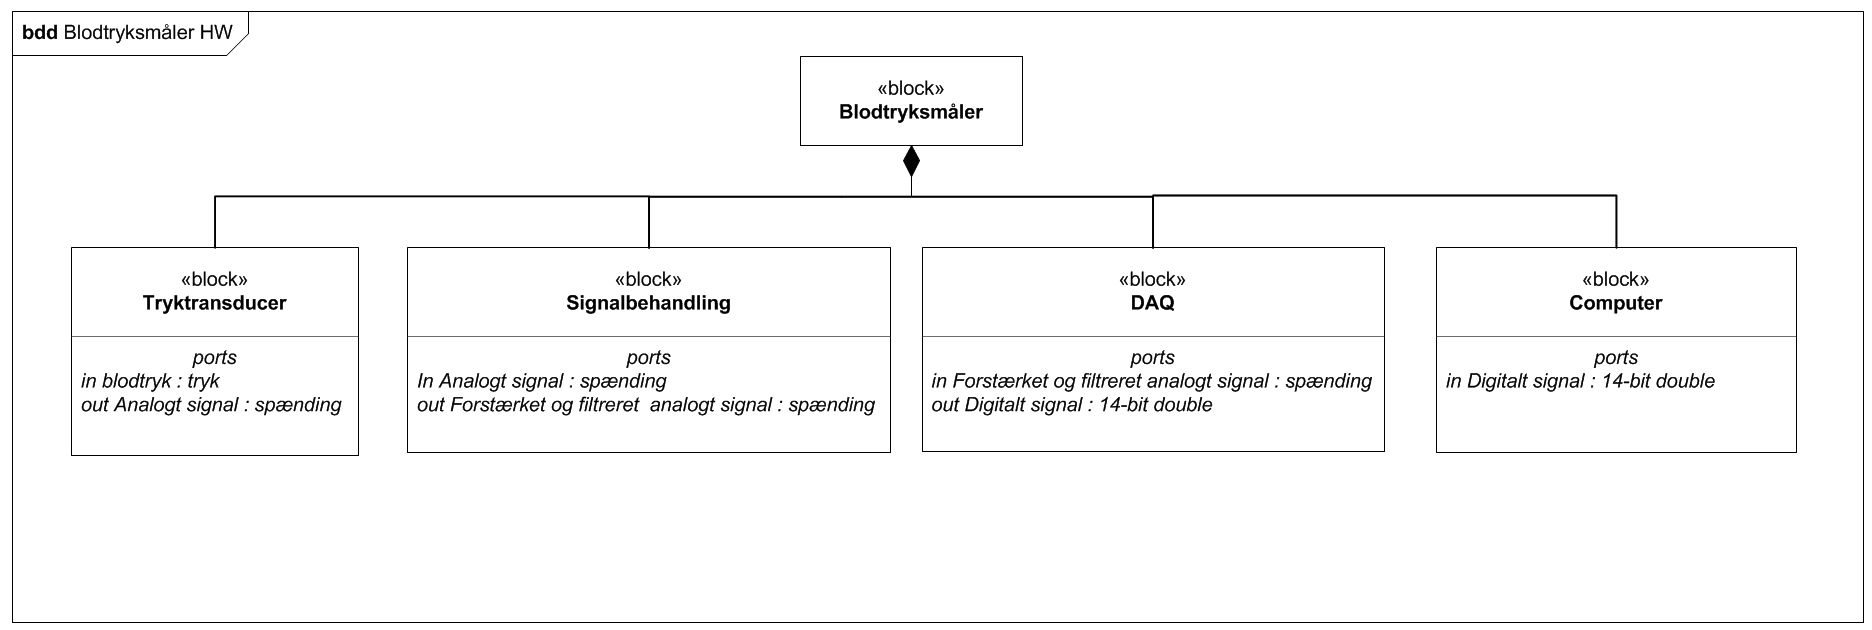
\includegraphics[width=1\textwidth]{Figurer/Snip20151209_70}
	\caption{bdd}
	\label{fig:bdd}
\end{figure}

\begin{longtabu} to \linewidth{@{}l X[j]@{}}
	\textbf{Blok} &	\textbf{Beskrivelse} \\[-1ex]
	\midrule
	Blodtryksmåler & Det overordnede system, som indeholder Tryktransducer, Signalbehandling, DAQ og Computer.\\[-1ex]
	Tryktransducer & Registrerer en fysisk størrelse i form af en trykændring. Tryktransduceren har til opgave at transformere den fysiske størrelse til en elektrisk spænding, som viderebehandles gennem de resterende hardwareblokke.  \\[-1ex]
	Signalbehandling & Består af to dele. En forstærkerdel og en filteringsdel. Det analoge signal fra Tryktransduceren bliver via denne blok forstærket og filteret.\\[-1ex]
	DAQ & Konverterer det forstærkede og filterede analoge signal til et digitalt signal. Der er valgt et spændingsområde fra +/- 5 V.\\[-1ex]
	Computer & Indeholder software til systemet, som er kodet i Visual Studio C\#. Softwaren kan blandt andet vise det digitale signal grafisk. Softwaren kan ligeledes kalibrere, nulpunktsjustere og gemme målinger samt aktivere og deaktivere filter.\\[-1ex]
	\caption{Beskrivelse af blokkene for systemet}
	\end{longtabu}
	
\subsection{ibd}
På Figur 2.2 ses et ibd for systemet. Ibd viser, hvordan de forskellige hardwareblokke interagerer med hinanden. Ibd fortæller signalets behandling gennem systemet - altså hvordan signalet transformeres fra et målt fysisk tryk til et digitalt signal, som softwaren kan viderebehandle og vise grafisk. 

\begin{figure}[H]
	\centering
	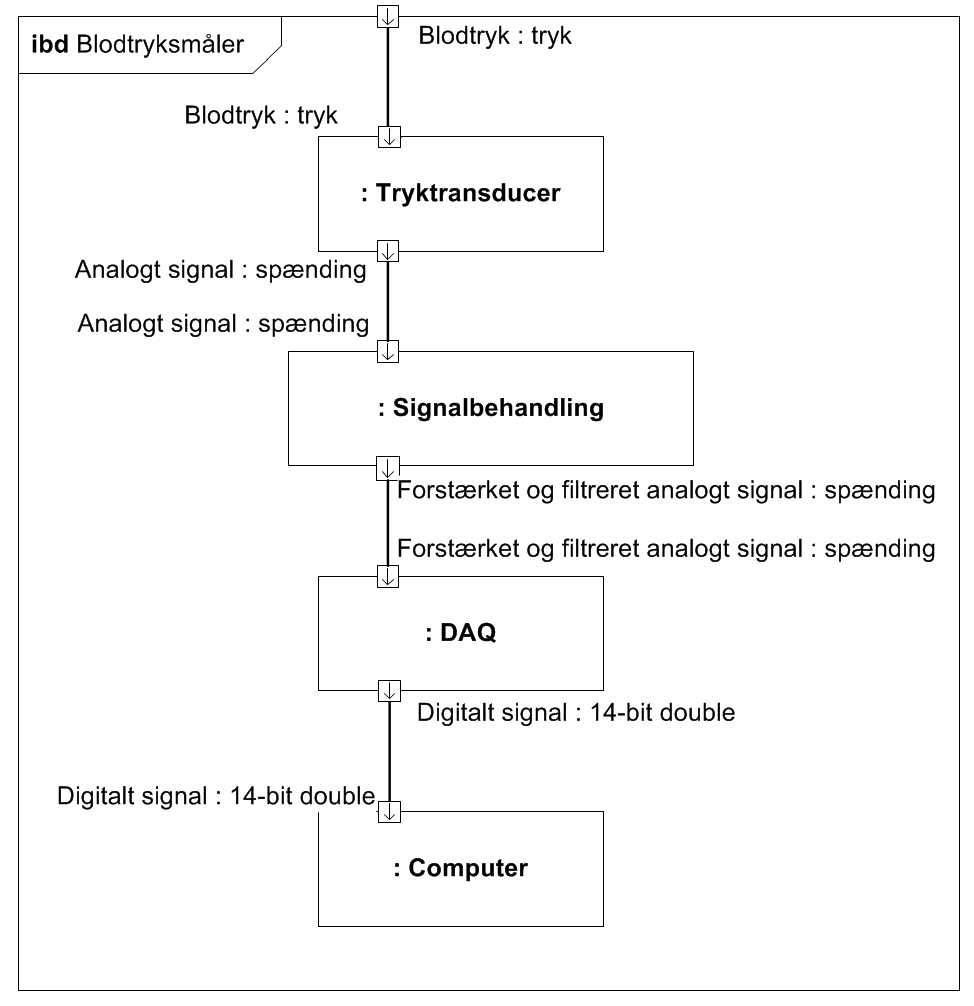
\includegraphics[width=0.8\textwidth]{Figurer/Snip20151209_72}
	\caption{ibd}
	\label{fig:ibd}
\end{figure}

\section{Grænseflader}
Kommunikationsprotokol for hardwareblokkene ses i Tabel 2.3. Det er en beskrivelse og specifikation af hvilket input- og outputsignal, de forskellige hardwareblokke har. 
\\  \\
Tryktransducerens maksimale output, $V_{max}$, bestemmes ud fra følgende ligning:

\begin{equation}
	V_{max} = P \cdot K \cdot V_{+}
\end{equation}

P = Tryk\\
K = sensitivitet\\
$V_{+}$ = inputspænding\\

For systemet er der valgt, at Tryktransducerens målbare område skal ligge i intervallet 0-300 mmHg. Den maksimale outputspænding bliver derfor udtrykt ved det maksimale tryk på 300 mmHg, sensitiviteten på 5 $\mu$ og inputspændingen på 5 V. Inputspændingen kommer reelt fra 9 V's batterier, men der er valgt at indsætte en 5 V regulator, så man er sikker på, hvad inputspændingen er, da batterier kan være ustabile.  


\begin{equation}
	V_{max} = 300  mmHg \cdot 5\mu V \cdot 5 V\\
\end{equation}
\begin{equation}
	V_{max} = 7,5 mV
\end{equation}


  

\begin{longtabu} to \linewidth{@{}l l l l X[j]@{}}
	\textbf{Grænseflade} & \textbf{Signal} & \textbf{Type} & \textbf{Format} & \textbf{Værdi} \\[-1ex]
	\midrule
	Tryktransducer & Blodtryk & in & Tryk & 0 - 300 mmHg \\[-1ex]
				& Analogt & out & Spænding & +/- 7,5 mV \\[-1ex]
	Signalbehandling  & Analogt & in & Spænding & +/- 7,5 mV \\[-1ex]
			 & Forstærket og filteret analogt & out & Spænding & +/- 5 V \\[-1ex]
	DAQ			& Forstærket og filteret analogt & in & Spænding & +/- 5 V \\[-1ex]	
				& Digitalt & out & 14-bit double & 0-5 V \\[-1ex]
	Computer	& Digitalt & in & 14-bit double &  0-5 V \\[-1ex]
	\caption{Kommunikationsprotokol}	
\end{longtabu}


\section{Hardware arkitektur}
Herunder er de krævede specifikationer for Signalbehandlingsblokken beskrevet. Tryktransduceren beskrives ligeledes, da denne har indflydelse for Forstærkerblokkens specifikationer. 

\subsubsection{Tryktransducer}
Tryktransduceren skal omsætte det fysiske tryk til en elektrisk spænding. Tryktransduceren har en meget høj common mode rejection samt en høj sensitivitet på 5 $\mu$V/V/mmHg +/- 1 \% \footnote{Se datablad for Tryktransduceren i bilag} , da de forventede trykændringer er små. Enheden for sensitiviteten angiver, hvor mange $\mu$V output der kommer fra Tryktransduceren pr. antal V i Tryktransducerens eksitationsspænding pr. mmHg. For at være sikker på at strømmen igennem Wheatstone broen ikke bliver for høj, og dermed i sidst ende kan brænde strain gauges af, er der blevet valgt at indsætte en regulator, der omdanner eksitationsspænding fra 9 V batterier til 5 V. 

\subsubsection{Forstærkerblok}
Forstærkerblokken sørger for at det svage spændingssignal fra Tryktransduceren bliver forstærket til en spænding, der ligger indenfor det måleinterval, der svarer til DAQ'ens, som er valgt til +/- 5 V.
 
\subsubsection{Filterblok}
Filterets formål er at frasortere blodtrykssignalets frekvenser, der er højere end 50 Hz, da disse ikke har nogen relevans for blodtrykssignalet. Dette skal realiseres ved et anden ordens lavpasfilter. 
 
\subsection{bdd}
På Figur 2.3 ses et bdd for Signalbehandlingsblokken, hvor Forstærkerblokkens og Filterblokkens input- og outputporte er vist.  
\begin{figure}[H]
	\centering
	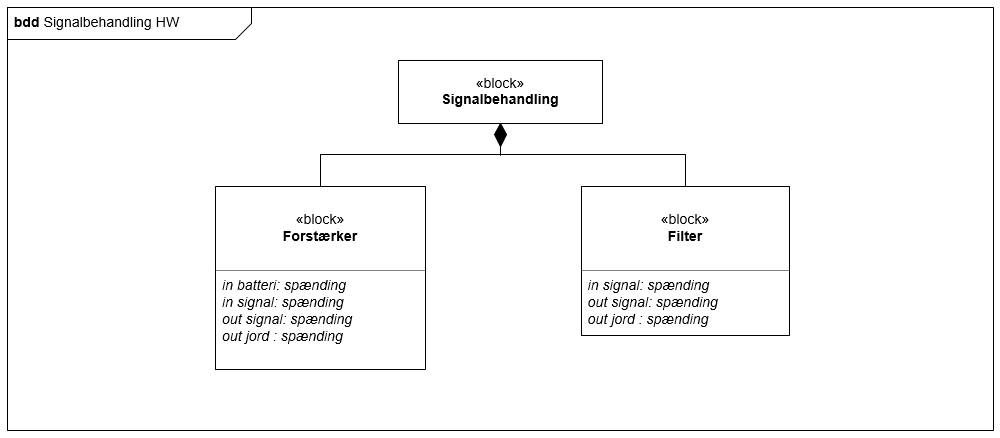
\includegraphics[width=1\textwidth]{Figurer/4}
	\caption{bdd for Signalbehandling HW}
	\label{fig:bdd hw}
\end{figure}

\subsection{Ibd}
På Figur 2.4 ses et ibd for Signalbehandlingsblokken. Ibd viser, hvordan Forstærkerblokken og Filterblokken interagerer med hinanden. 

\begin{figure}[H]
	\centering
	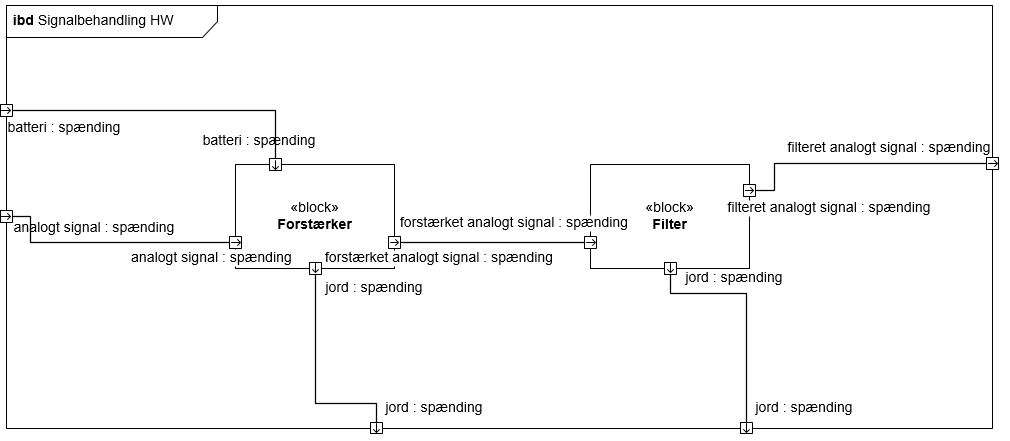
\includegraphics[width=1\textwidth]{Figurer/5}
	\caption{ibd for Signalbehandling HW}
	\label{fig:ibd hw}
\end{figure}

\subsection{Grænseflader}

\begin{longtabu} to \linewidth{@{}l l l l X[j]@{}}
	\textbf{Grænseflade} & \textbf{Signal} & \textbf{Type} & \textbf{Format} & \textbf{Værdi} \\[-1ex]
	\midrule
	Forstærker & Batteri & in & Spænding & +/- 9 V \\[-1ex]
			   & Analogt & in & Spænding & +/- 7,5 mV \\[-1ex]
			   & Jord	 & out & Spænding & 0 V \\[-1ex]
			   & Forstærket analogt & out & Spænding & +/- 5 V \\[-1ex]
	Filter	   & Forstærket analogt & in & Spænding & +/- 5 V\\[-1ex]
			   & Jord	 & out & Spænding & 0 V\\[-1ex]
			   & Filteret analogt & out & Spænding & +/- 5 V\\[-1ex]
	\caption{Kommunikationsprotokol for Signalbehandlingsblok}	
\end{longtabu}


 \subsection{Forstærkerblok}
 \subsubsection{Specifikationer}
 \begin{itemize}
 	\item Forstærkningen, gain, skal forstærke den maksimale inputspænding, så outputtet bliver 10 V
 	\begin{equation}
 		Gain \cdot V_{in} = V_{out}
 	\end{equation}
 	
 	$V_{out}$ og $V_{in}$ er kendt, så gain isoleres
 	
 	\begin{equation}
 		Gain = \frac{V_{out}}{V_{in}} \\ \Longrightarrow \\
 		Gain = \frac{5000 mV}{7,5 mV}\\ \Longrightarrow \\
 		Gain = 666,667
 	\end{equation}
 	
 	
 	
 	\item Inputspænding: +/- 7,5 mV
 	\item Eksitationsspænding: +/- 9 V
 	\item Outputspænding: +/- 5 V
 	\item Minimum en båndbredde på 50 Hz
 	\item Uendelig indgangsimpedans i teorien
 \end{itemize}


 \subsection{Filterblok}
 \subsubsection{Specifikationer}
 \begin{itemize}
 	\item Anden ordens lavpasfilter
 	\item Cutoff frekvens ved 50 Hz
 	\item Unity gain (ingen forstærkning)
 	\item -40 dB ved 500 Hz
 	\item Uendelig indgangsimpedans i teorien
 	\item Inputspænding +/- 5 V
 	\item Eksitationsspænding +/- 9 V
 \end{itemize}
 

\section{Software arkitektur}

\subsection{Domænemodel}
Domænemodellen er skabt på baggrund af de seks Use Cases og fungerer som et middel til at skabe et samlet overblik over systemet. Gennem navneordsanalyse er de konceptuelle klasser fundet. I modellen beskrives, hvordan de konceptuelle klasser og aktører interagerer med hinanden. Controlleren er ikke en konceptuel klasse, men den sørger for, at systemet fungerer optimalt og udfører kommandoer.

\begin{figure}[H]
	\centering
	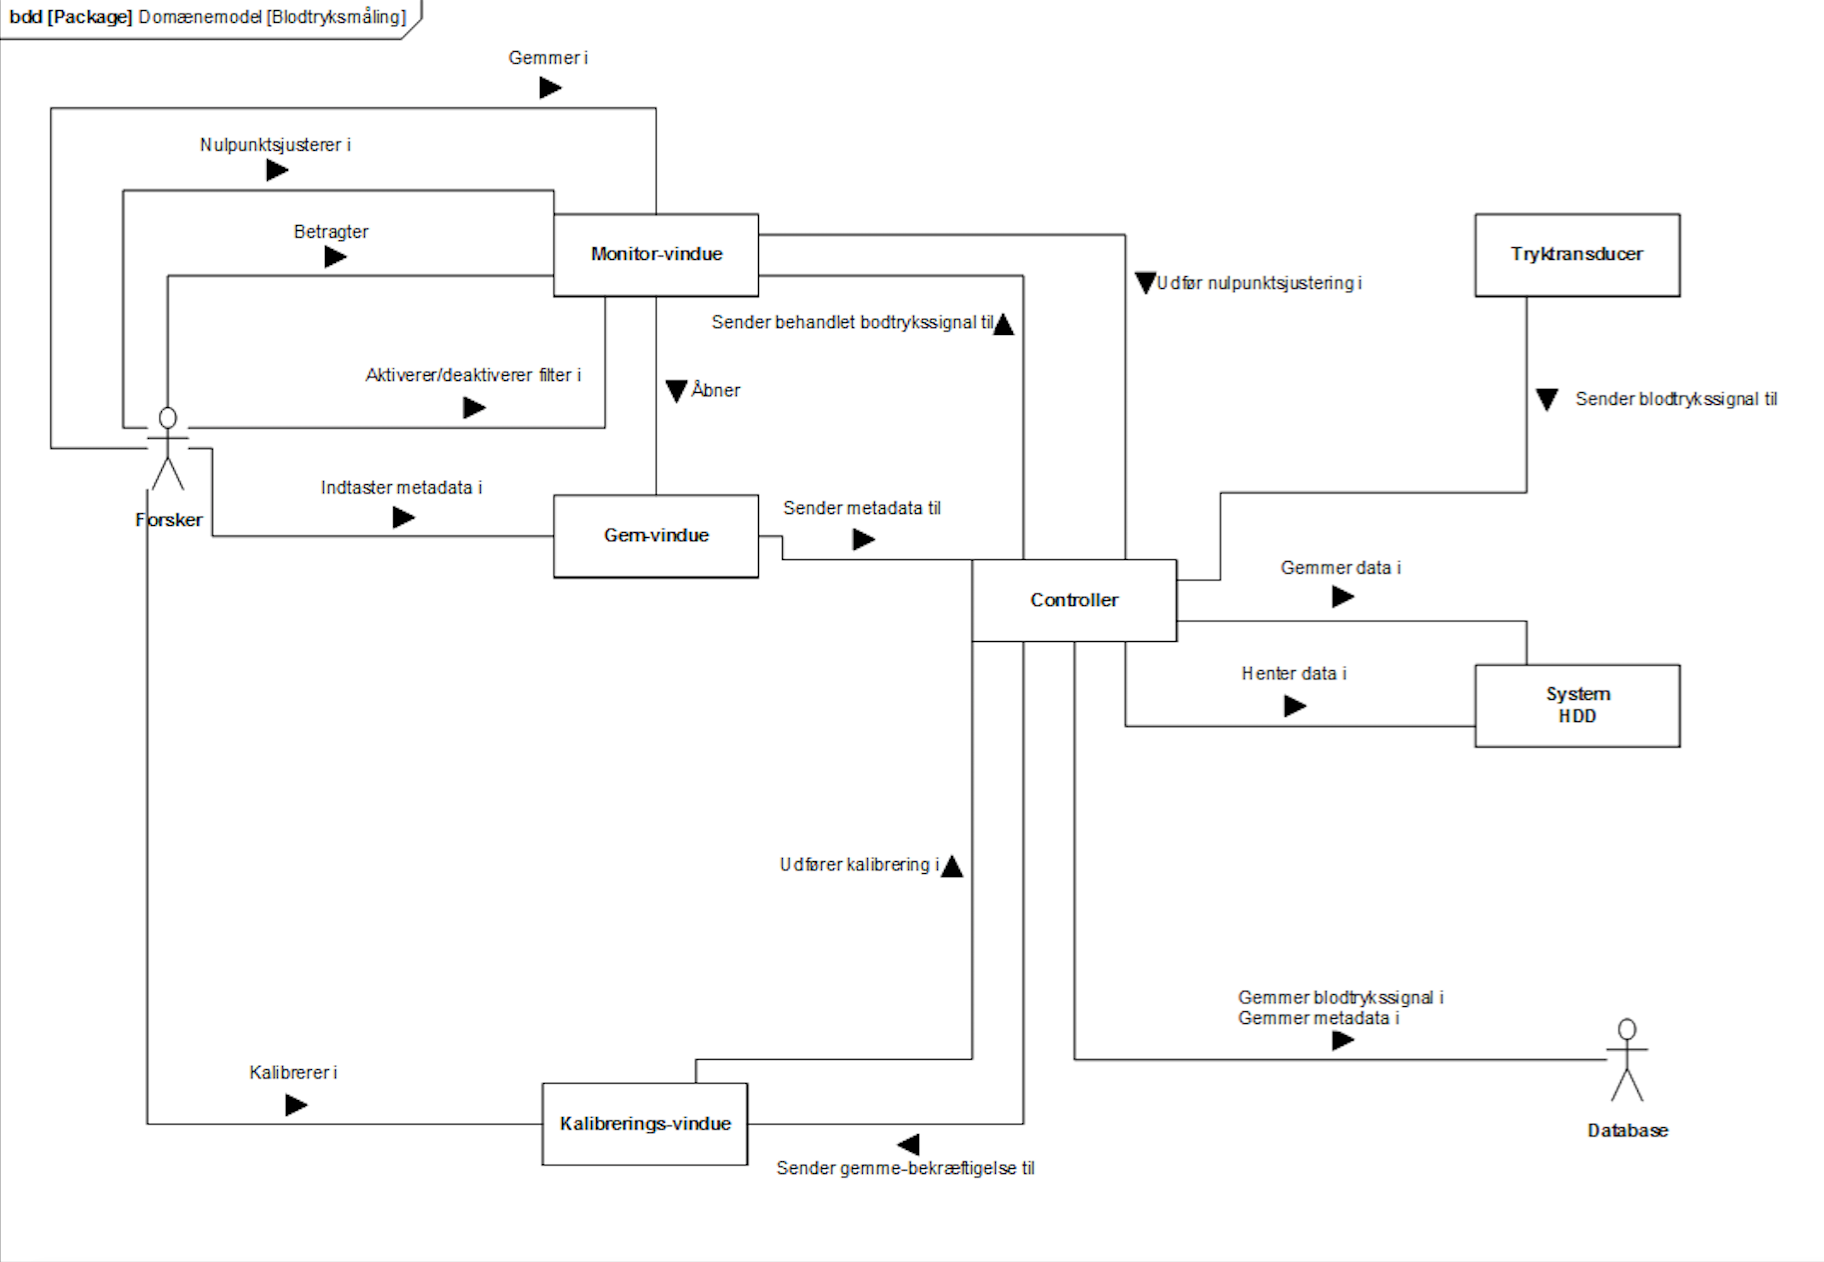
\includegraphics[width=1 \textwidth]{Figurer/screenshot}
	\caption{Domænemodel for blodtryksmålesystemet}
\end{figure}
I domænemodellen ses generelle principper om kommunikation mellem klasser og aktører. Kommunikationen kan derfor være af forskellig karakter, og funktionaliteten af den givne kommando kan variere fra Use Case til Use Case.

\subsection{Applikationsmodel}

\subsubsection{Sekvensdiagram}
Sekvensdiagrammerne beskriver step-by-step forløbet i de forskellige Use Cases via metoder. Der er lavet et sekvensdiagram for hver Use Case for at gøre systemet mere overskueligt. Et sekvensdiagram består af boundary-klasserne og domain-klasserne fra domænemodellen, samt en controller-klasse, med navn efter den specifikke Use Case.

\begin{figure}[H]
	\centering
	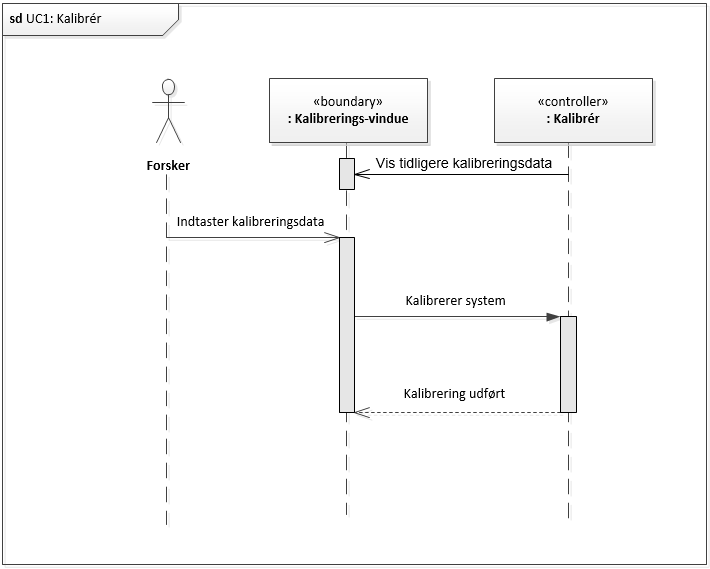
\includegraphics[width=1\textwidth]{Figurer/UC1_SD}
	\caption{Sekvensdiagram for Use Case 1}
\end{figure}

Forsker interagerer med Monitor-vindue. Kalibreringsmetoden bliver kaldt, når Forsker trykker på knappen ”Ja”. Derefter igangsættes kalibreringen og kalibrerings-tidspunkt, og værdi sendes og gemmes i Databasen. 

\begin{figure}[H]
	\centering
	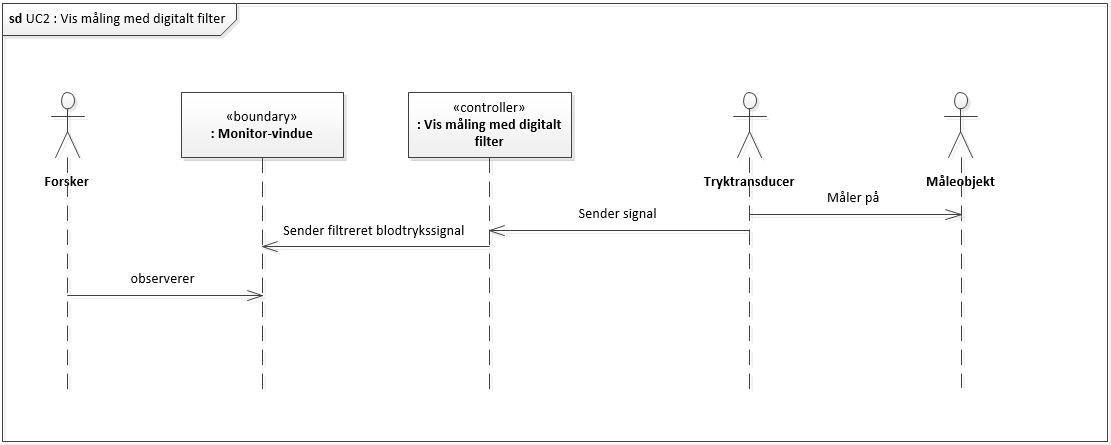
\includegraphics[width=1\textwidth]{Figurer/UC2_SD}
	\caption{Sekvensdiagram for Use Case 2}
\end{figure}

Controller henter data fra Tryktransducer, som henter data i form af tryk fra Måleobjekt. Datafilerne sendes fra Måleobjekt via Tryktransducer tilbage til Controller, der kalder en metode. Monitor-vinduet opdateres, og herefter kan Forsker aflæse blodtryk. 

\begin{figure}[H]
	\centering
	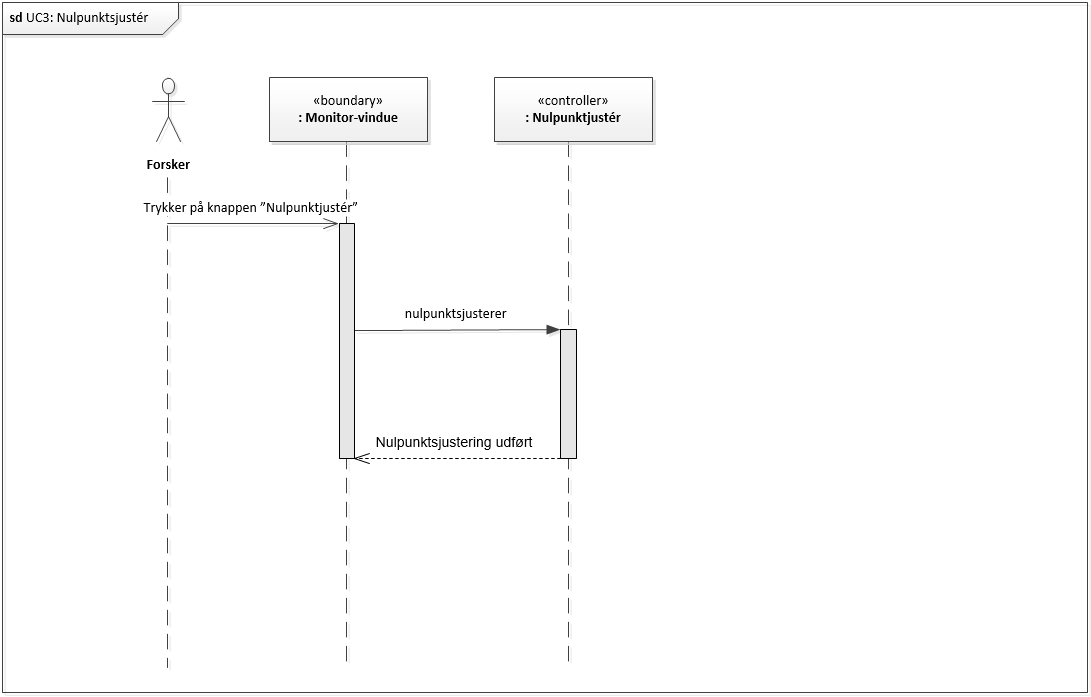
\includegraphics[width=1\textwidth]{Figurer/UC3_SD}
	\caption{Sekvensdiagram for Use Case 3}
\end{figure}

Forsker interagerer med Monitor-vinduet ved at trykke på knappen ”Nulpunktsjustér”. Derefter kaldes en metode, og nulpunktsjusteringen startes. Tidspunktet og værdien for nulpunktjusteringen sendes og gemmes i Databasen, hvorefter Forsker får besked om, at nulpunktsjusteringen er foretaget. 

\begin{figure}[H]
	\centering
	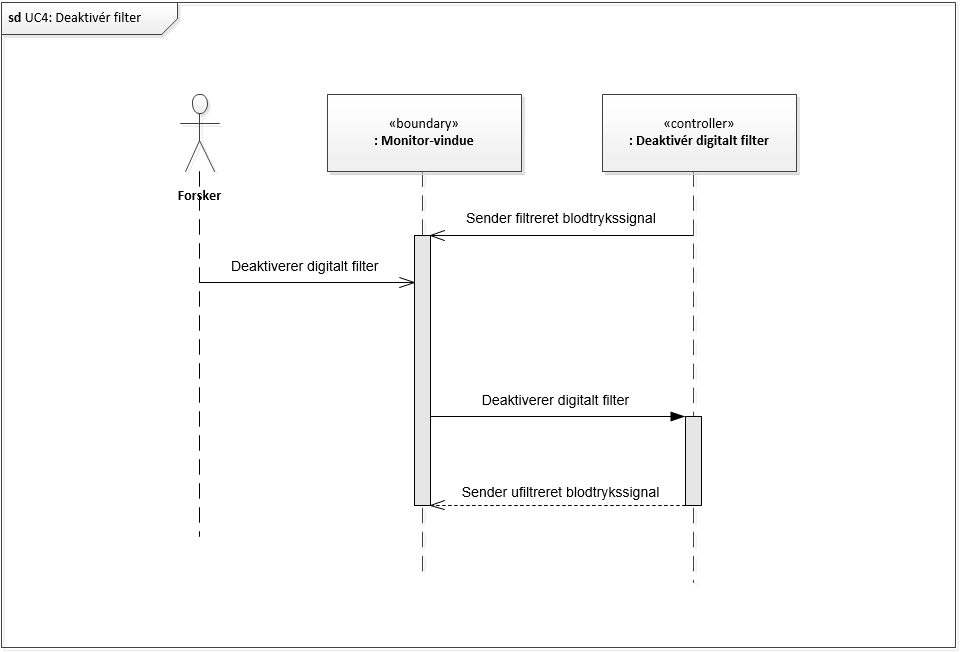
\includegraphics[width=1\textwidth]{Figurer/UC4_SD}
	\caption{Sekvensdiagram for Use Case 4}
\end{figure}

Forsker interagerer med Monitor-vinduet ved at markere "Off"\--radiobutton under "Filter". Derefter kaldes en metode, og filteret deaktiveres, hvorefter signalet bliver udskrevet ufiltreret.

\begin{figure}[H]
	\centering
	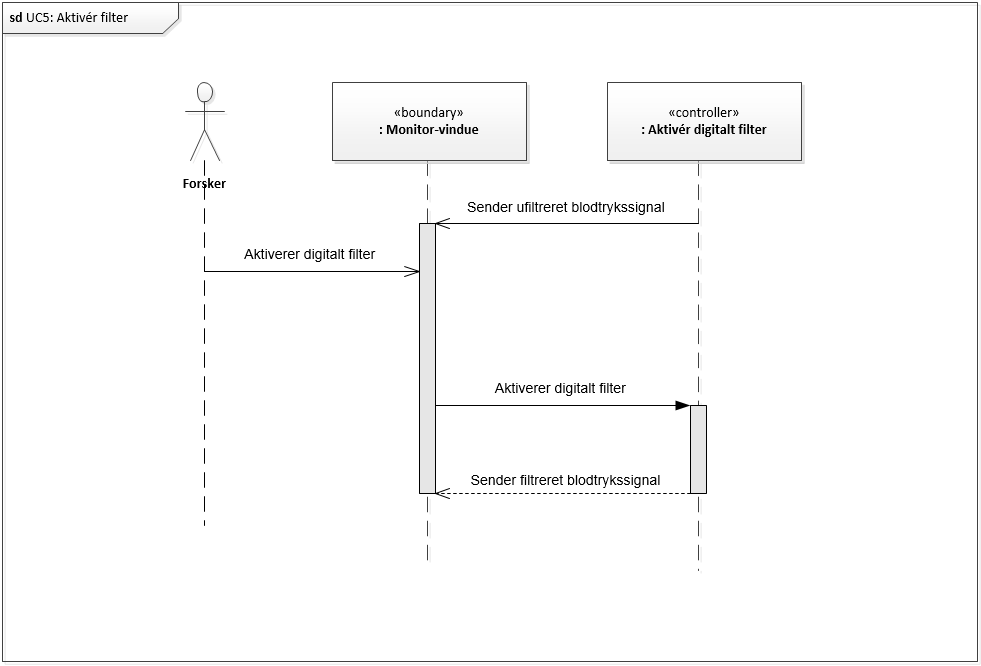
\includegraphics[width=1\textwidth]{Figurer/UC5_SD}
	\caption{Sekvensdiagram for Use Case 5}
\end{figure}

Forsker interagerer med Monitor-vinduet ved at markere "On"\--radiobutton under "Filter". Derefter kaldes en metode, og filteret aktiveres, hvorefter signalet bliver udskrevet filtreret.

\begin{figure}[H]
	\centering
	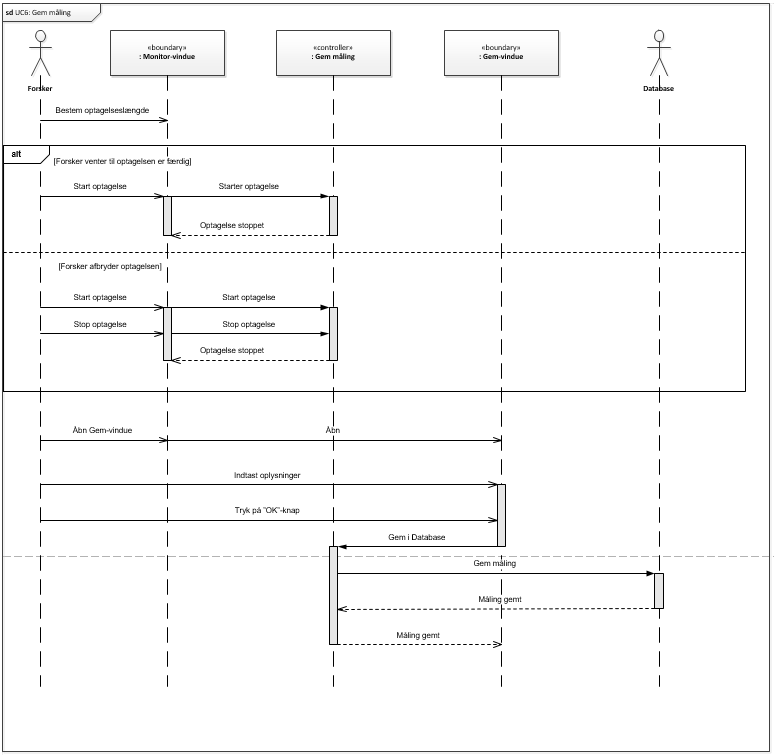
\includegraphics[width=1\textwidth]{Figurer/UC6_SD}
	\caption{Sekvensdiagram for Use Case 6}
\end{figure}

Forsker interagerer med Monitor-vinduet ved at trykke på knappen ”Gem”. Derefter kaldes en metode og Gem-vinduet åbnes. Når Forsker ønsker at gemme, indtastes data om målingen og der trykkes på knappen ”OK”. Kommando sendes og data gemmes. Controller bekræfter til Gem-vinduet, at data er gemt.
